% main.tex — JKCS (Journal of the Korean Ceramic Society) submission
% Springer Nature sn-jnl template
% NOTE: Switch to sn-jnl class when the correct version is available.
%       Current build uses article class for compatibility.
\documentclass[12pt,a4paper]{article}

%%% Packages %%%
\usepackage{graphicx}
\usepackage{multirow}
\usepackage{amsmath,amssymb,amsfonts}
\usepackage{booktabs}
\usepackage{siunitx}
\usepackage[colorlinks=true,linkcolor=blue,citecolor=blue]{hyperref}
\usepackage[margin=25mm]{geometry}

%%% SI units setup %%%
\sisetup{
  per-mode=symbol,
  inter-unit-product=\ensuremath{\cdot},
}

\begin{document}

\title{Bayesian Optimization of Gyroid TPMS Catalyst Support Geometry
  for Pressure Drop and Surface Area Using Lattice Boltzmann Method}

\author{Hyun-Kyu Tae\footnote{Corresponding author. E-mail: thk@example.com} \\
  \small Affiliation TBD, Republic of Korea}

\date{}
\maketitle

\begin{abstract}
Triply periodic minimal surface (TPMS) structures, particularly the gyroid,
have attracted attention as catalyst supports due to their high surface-area-to-volume
ratio and tunable porosity. In this study, we apply Bayesian optimization (BO)
to the design of gyroid catalyst supports, exploring the unit-cell size $a$
and threshold parameter $t$ to balance specific surface area $S_v$ against
pressure drop $\Delta P$. A D3Q19 multiple-relaxation-time lattice Boltzmann
method (MRT-LBM) solver implemented in Taichi is used to evaluate
Darcy permeability $K$ for each candidate geometry. One hundred BO evaluations
yield 50 Pareto-optimal designs, from which five representative configurations
(A--E) are selected for detailed characterization, including GHSV-dependent
pressure loss, Forchheimer nonlinear regression, flow mixing metrics,
and numerical reproducibility analysis.  Results show that designs with
$a = 3$--$\SI{6}{\milli\meter}$ achieve $S_v > \SI{2000}{\per\meter}$
while maintaining $\Delta P < \SI{50}{\pascal}$ at the reference GHSV,
offering practical trade-offs for ceramic catalyst support applications.
\end{abstract}

\noindent\textbf{Keywords:} Gyroid; TPMS; Lattice Boltzmann method;
Bayesian optimization; Catalyst support; Permeability

\section{Introduction}\label{sec:intro}

Catalytic converters in automotive exhaust systems and industrial reactors
rely on porous support structures that must simultaneously provide
high catalytic surface area and low flow resistance.
Conventional honeycomb monoliths, while widely adopted, suffer from
limited radial mixing and anisotropic transport properties~\cite{ref_honeycomb}.

Triply periodic minimal surface (TPMS) structures have emerged as
promising alternatives owing to their mathematically defined,
fully interconnected pore networks~\cite{ref_tpms_review}.
Among TPMS families, the gyroid---described by the level-set function
\begin{equation}\label{eq:gyroid}
  \varphi(\mathbf{x}) =
    \sin\!\frac{2\pi x}{a}\cos\!\frac{2\pi y}{a}
  + \sin\!\frac{2\pi y}{a}\cos\!\frac{2\pi z}{a}
  + \sin\!\frac{2\pi z}{a}\cos\!\frac{2\pi x}{a}
  = t,
\end{equation}
where $a$ is the unit-cell size and $t$ the threshold parameter---has
attracted particular interest because of its zero mean curvature,
tunable porosity $\varepsilon$, and feasibility of fabrication via
additive manufacturing of ceramics~\cite{ref_gyroid_ceramic}.

The design of gyroid-based catalyst supports involves a trade-off
between specific surface area $S_v$ and pressure drop $\Delta P$.
Increasing $S_v$ enhances catalytic activity but raises flow resistance.
Bayesian optimization (BO) provides a sample-efficient strategy for
navigating such trade-offs when each function evaluation is
computationally expensive~\cite{ref_bo_review}.

The lattice Boltzmann method (LBM) is well-suited for simulating
flow through complex porous geometries due to its inherent parallelism
and straightforward handling of irregular boundaries~\cite{ref_lbm_porous}.
In this work, we couple a D3Q19 multiple-relaxation-time (MRT) LBM solver,
implemented on GPU via the Taichi programming framework~\cite{ref_taichi},
with a BO pipeline to systematically explore the $(a, t)$ design space
of gyroid catalyst supports.

The objectives of this study are:
\begin{enumerate}
  \item To establish a validated, GPU-accelerated LBM simulation framework
        for gyroid TPMS permeability evaluation;
  \item To identify Pareto-optimal designs that balance $S_v$ and $\Delta P$
        using BO with 100 evaluations;
  \item To characterize the selected designs in terms of Forchheimer
        nonlinear behavior, GHSV-dependent pressure loss, and flow
        mixing metrics.
\end{enumerate}

\section{Methods}\label{sec:methods}

\subsection{Gyroid Geometry}\label{sec:geom}

The gyroid surface is defined by Eq.~\eqref{eq:gyroid}.
The solid phase occupies the region $\varphi(\mathbf{x}) \ge t$,
where $t \in (-0.5,\; 0.5)$ controls wall thickness and porosity
$\varepsilon$.  The unit-cell size $a$ determines the characteristic
pore dimension.  For each $(a, t)$ pair, the voxelized domain is
constructed on a Cartesian grid with resolution $\Delta x = \SI{0.2}{\milli\meter}$,
yielding $N_x = N_y = 131$ and $N_z = 2a/\Delta x$.

The specific surface area $S_v$ (surface area per unit volume, \si{\per\meter})
and porosity $\varepsilon$ are computed directly from the voxelized geometry.

\subsection{Lattice Boltzmann Solver}\label{sec:lbm}

A D3Q19 MRT-LBM scheme is employed~\cite{ref_mrt_lbm}.
The solver is implemented in Taichi (v1.7.4) with CUDA backend.
Key simulation parameters are listed in Table~\ref{tab:lbm_params}.

\begin{table}[htbp]
\caption{LBM simulation parameters.}\label{tab:lbm_params}
\centering
\begin{tabular}{@{}lll@{}}
\toprule
Parameter & Symbol & Value \\
\midrule
Lattice & --- & D3Q19 \\
Collision model & --- & MRT \\
Grid resolution & $\Delta x$ & \SI{0.2}{\milli\meter} \\
Domain (cross-section) & $N_x \times N_y$ & $131 \times 131$ \\
Domain (streamwise) & $N_z$ & $2a/\Delta x$ \\
Boundary condition & --- & Periodic + body force \\
Framework & --- & Taichi 1.7.4, \texttt{arch=cuda} \\
\bottomrule
\end{tabular}
\end{table}

The no-slip condition at solid walls is enforced via the bounce-back scheme.
Periodic boundary conditions are applied in the streamwise ($z$) direction,
and a uniform body force $g_\mathrm{lbm}$ drives the flow.
Darcy permeability is obtained from the steady-state velocity field:
\begin{equation}\label{eq:darcy}
  K = \frac{\mu \, \langle u_z \rangle}{(\Delta P / L)},
\end{equation}
where $\mu$ is the dynamic viscosity, $\langle u_z \rangle$ the
volume-averaged streamwise velocity, and $L$ the domain length.

\subsection{Bayesian Optimization}\label{sec:bo}

The BO framework uses Gaussian process regression with the
Lower Confidence Bound (LCB) acquisition function
($\kappa = 3$)~\cite{ref_bo_lcb}, implemented via
\texttt{scikit-optimize}.  The design space is:

\begin{table}[htbp]
\caption{Bayesian optimization configuration.}\label{tab:bo_config}
\centering
\begin{tabular}{@{}ll@{}}
\toprule
Parameter & Value \\
\midrule
Design variable $a$ & $[\num{3.0},\; \num{12.0}]$ \si{\milli\meter} \\
Design variable $t$ & $(-0.5,\; 0.5)$ \\
Acquisition function & LCB, $\kappa = 3$ \\
Initial samples & 20 (random) \\
Iterations & 80 \\
Total evaluations & 100 \\
\bottomrule
\end{tabular}
\end{table}

The objective is to minimize $\Delta P_\mathrm{Darcy}$
while simultaneously maximizing $S_v$.
A design is marked \emph{feasible} if the simulation converges
and satisfies physical consistency checks.

\subsection{Post-processing}\label{sec:postproc}

\paragraph{Forchheimer analysis.}
For the top-5 designs, five body-force levels
($g_\mathrm{lbm} \in \{10^{-6},\; 5{\times}10^{-6},\; 5{\times}10^{-5},\;
5{\times}10^{-4},\; 2{\times}10^{-3}\}$) are applied.
The extended Darcy--Forchheimer equation,
\begin{equation}\label{eq:forch}
  \frac{\Delta P / L}{u} = \frac{\mu}{K} + \beta\,\rho\,u,
\end{equation}
is fitted via linear regression of $(\Delta P/L)/u$ versus $u$
to extract permeability $K$ and inertial coefficient $\beta$.

\paragraph{Flow metrics.}
Mixing ratio ($v_\mathrm{trans}/|v_z|$), velocity uniformity
($\sigma_{v_z}$), and hydraulic tortuosity $\tau$ are evaluated
at the mid-plane cross-section.

\paragraph{GHSV sweep.}
Pressure drop at five gas hourly space velocities
(GHSV $= 5000$--$\num{60000}\;\si{\per\hour}$) is computed
from the Darcy relation $\Delta P = u_\mathrm{in}\,\mu\,L_\mathrm{cat}/K$.

\section{Results}\label{sec:results}

\subsection{Bayesian Optimization Convergence}\label{sec:bo_results}

Of 100 BO evaluations, 85 designs were feasible (OK) and 15 failed,
predominantly near the threshold boundary $|t| \approx 0.5$.
The unit-cell size $a$ spanned the full design range
($\num{3.0}$--$\SI{12.0}{\milli\meter}$, mean $\approx \SI{7.8}{\milli\meter}$),
and the specific surface area ranged from
$S_v \approx 770$ to $\SI{4491}{\per\meter}$.
% Fig.~\ref{fig:bo_convergence} shows the BO convergence history.

\subsection{Pareto Front and Top-5 Selection}\label{sec:pareto}

The multi-objective analysis yielded \textbf{50 Pareto-optimal points}
in the $S_v$--$\Delta P$ space (Fig.~\ref{fig:pareto}),
far exceeding the planned threshold of 15.
Five representative designs (A--E) were selected based on distinct criteria
(Table~\ref{tab:top5}).

\begin{figure}[htbp]
  \centering
  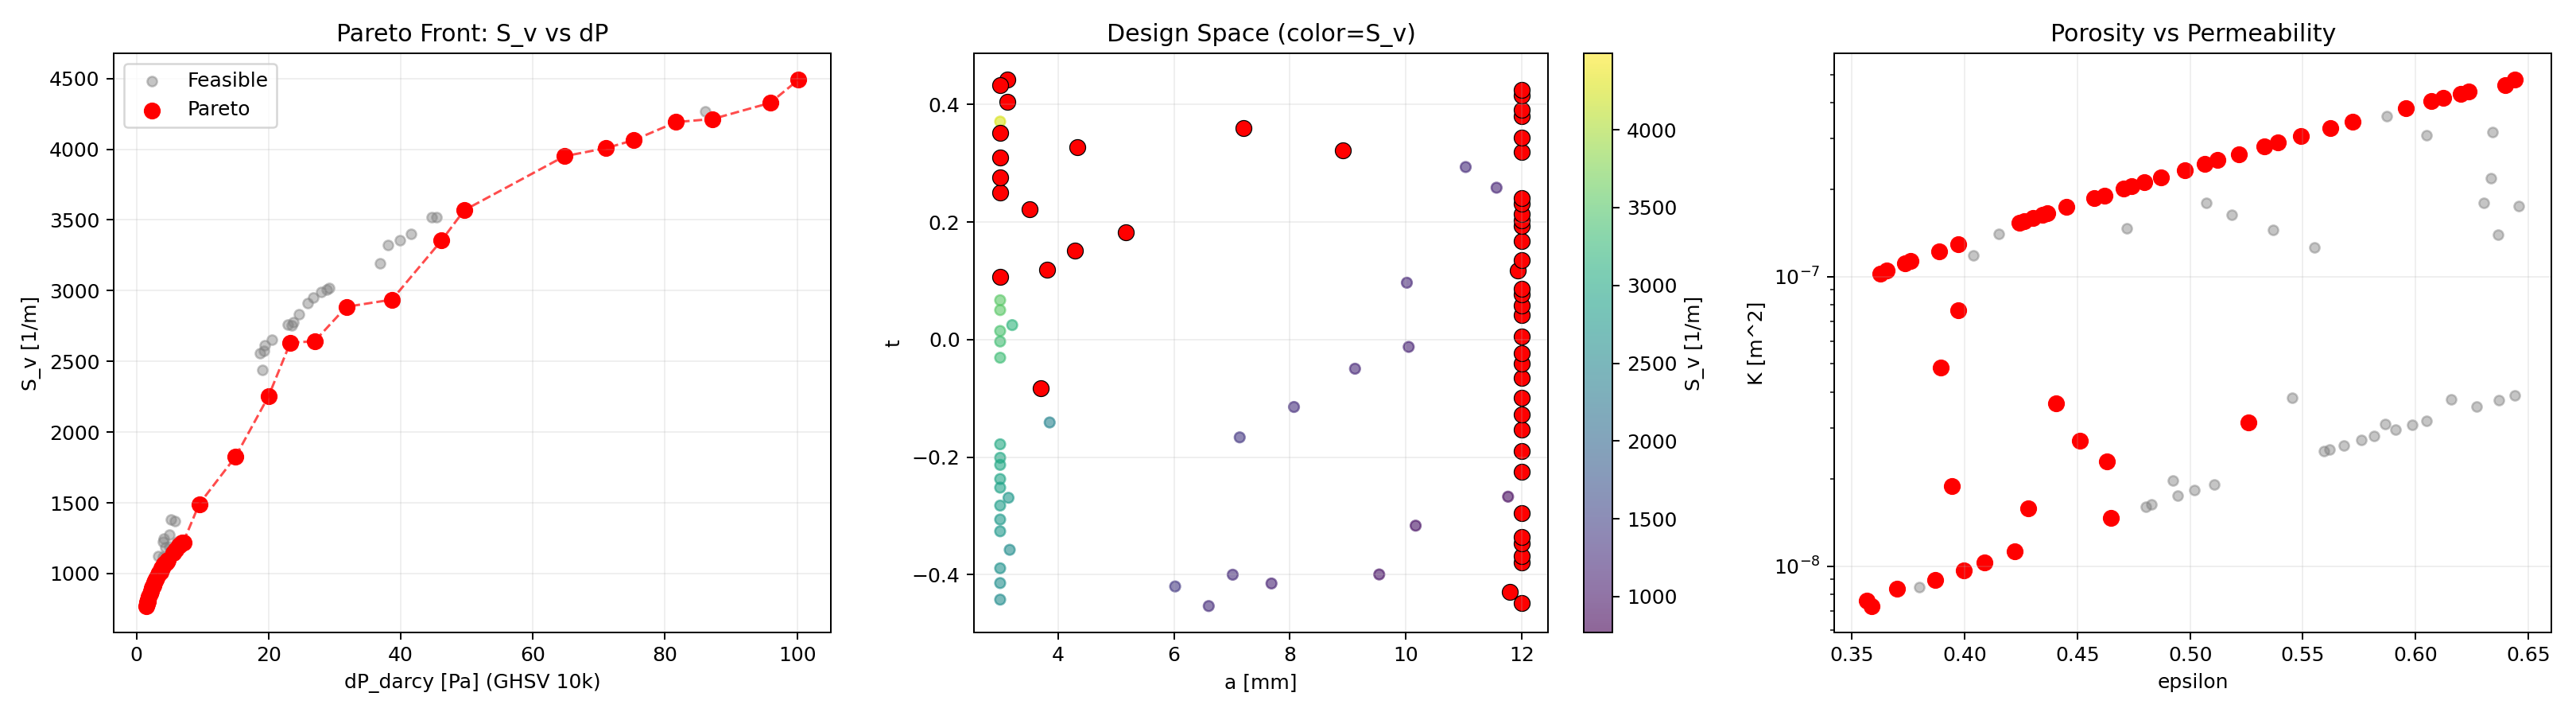
\includegraphics[width=0.85\linewidth]{figures/fig3_pareto_front.png}
  \caption{Pareto front in the $S_v$--$\Delta P$ design space.
           50 non-dominated points are identified from 85 feasible evaluations.}
  \label{fig:pareto}
\end{figure}

\begin{table}[htbp]
\caption{Top-5 selected designs from the Pareto front.}\label{tab:top5}
\centering
\begin{tabular}{@{}lccccccl@{}}
\toprule
Design & $a$ [\si{\milli\meter}] & $t$ & $\varepsilon$ &
  $S_v$ [\si{\per\meter}] & $K$ [\si{\meter\squared}] &
  $\Delta P$ [\si{\pascal}] & Criterion \\
\midrule
A & 3.00  &  0.433 & 0.359 & 4491 & \num{7.28e-9}  & 100.2 & Max $S_v$ \\
B & 12.00 & $-$0.449 & 0.644 & 770  & \num{4.79e-7}  & 1.5   & Min $\Delta P$ \\
C & 3.70  & $-$0.082 & 0.526 & 2632 & \num{3.13e-8}  & 23.3  & TOPSIS balanced \\
D & 3.00  &  0.107 & 0.465 & 3568 & \num{1.47e-8}  & 49.6  & $\varepsilon{\approx}0.5$, max $S_v$ \\
E & 5.17  &  0.183 & 0.441 & 2252 & \num{3.65e-8}  & 20.0  & Manufacturability \\
\bottomrule
\end{tabular}
\end{table}

\subsection{Flow Visualization}\label{sec:flow_vis}

Figure~\ref{fig:velocity} shows the streamwise velocity ($v_z$) contours
at the mid-plane cross-section for designs A, C, and E.
Design~A, with the smallest unit cell ($a = \SI{3}{\milli\meter}$),
exhibits the finest flow channeling pattern and strongest transverse mixing.

\begin{figure}[htbp]
  \centering
  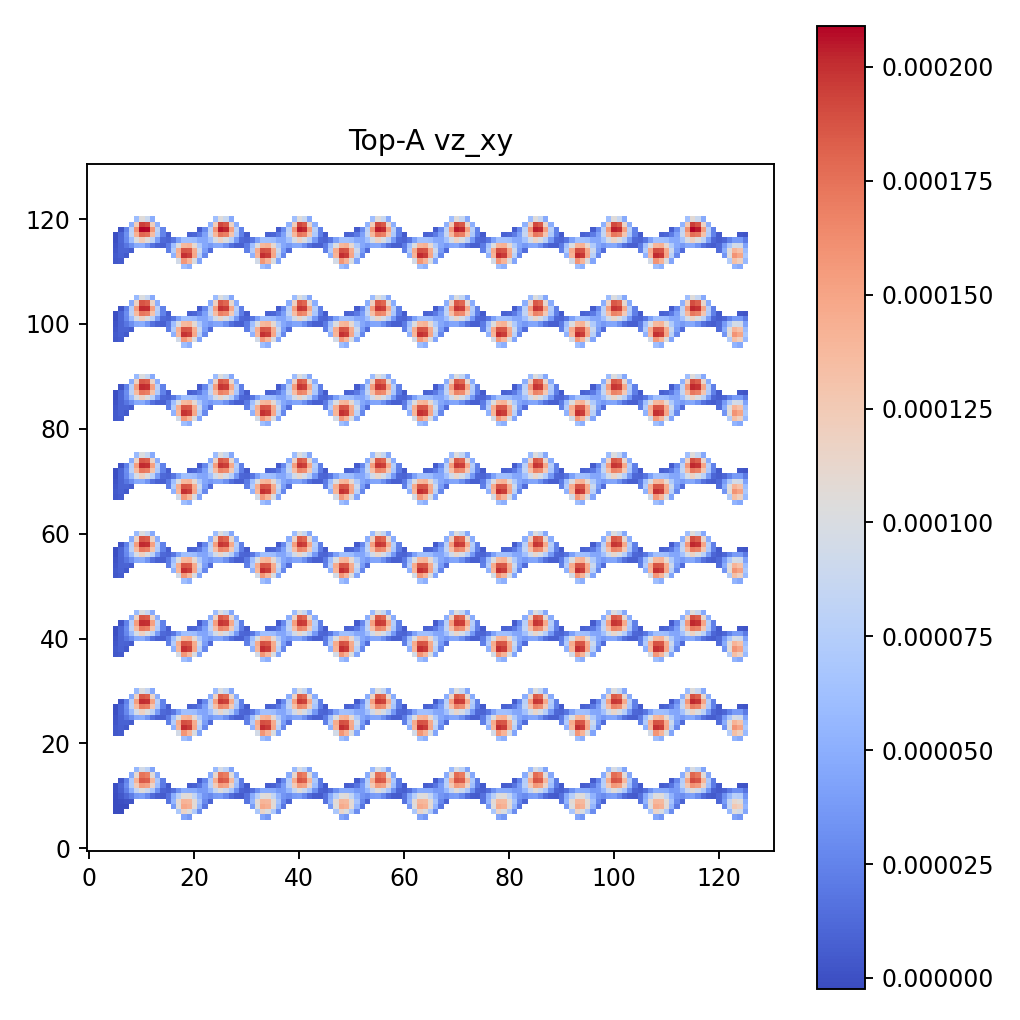
\includegraphics[width=0.32\linewidth]{figures/fig4a_vz_xy_A.png}
  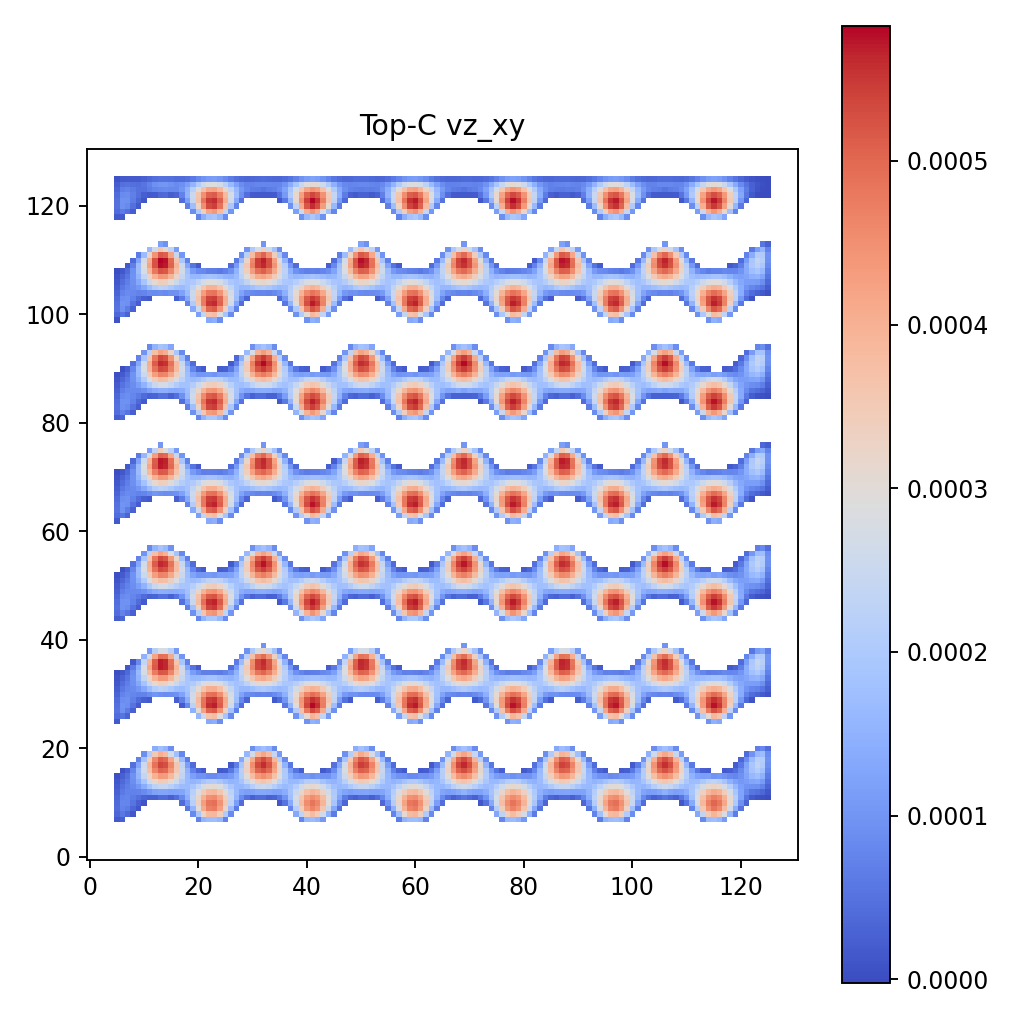
\includegraphics[width=0.32\linewidth]{figures/fig4b_vz_xy_C.png}
  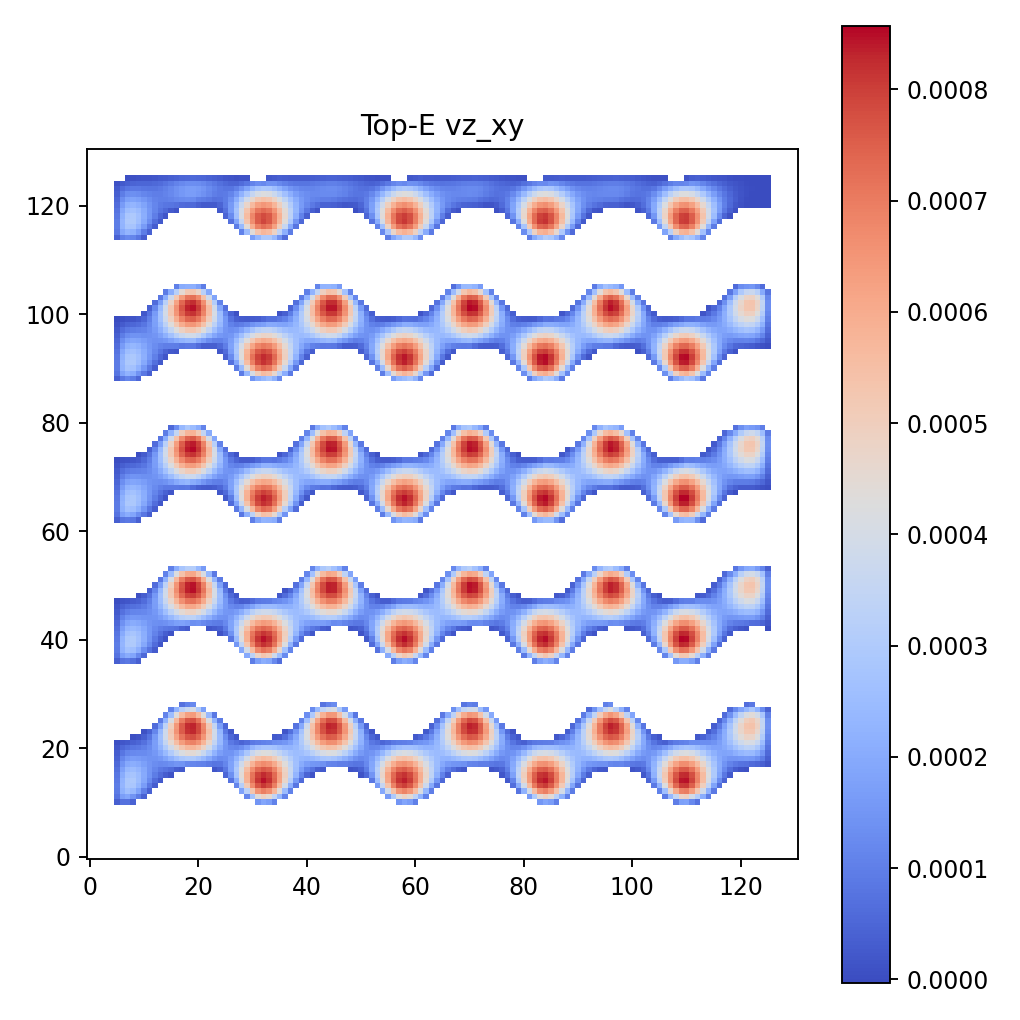
\includegraphics[width=0.32\linewidth]{figures/fig4c_vz_xy_E.png}
  \caption{Streamwise velocity $v_z$ at the mid-plane for designs
           A (left), C (center), and E (right).}
  \label{fig:velocity}
\end{figure}

\subsection{GHSV Sensitivity}\label{sec:ghsv}

Table~\ref{tab:ghsv} summarizes the Darcy-estimated pressure drop
at five GHSV conditions for all five designs.
Design~B maintains $\Delta P < \SI{10}{\pascal}$ even at
GHSV $= \SI{60000}{\per\hour}$, while design~A reaches
$\approx \SI{601}{\pascal}$ at the same condition.

\begin{table}[htbp]
\caption{Pressure drop $\Delta P$ [\si{\pascal}] at various GHSV for Top-5 designs.}\label{tab:ghsv}
\centering
\begin{tabular}{@{}lccccc@{}}
\toprule
GHSV [\si{\per\hour}] & A & B & C & D & E \\
\midrule
5\,000   & 50.1  & 0.76  & 11.7  & 24.8  & 10.0 \\
10\,000  & 100.3 & 1.52  & 23.3  & 49.6  & 20.0 \\
20\,000  & 200.5 & 3.05  & 46.6  & 99.3  & 40.0 \\
40\,000  & 400.7 & 6.09  & 93.2  & 198.4 & 79.9 \\
60\,000  & 601.2 & 9.14  & 139.8 & 297.7 & 119.9 \\
\bottomrule
\end{tabular}
\end{table}

\subsection{Forchheimer Analysis}\label{sec:forch}

Table~\ref{tab:forch} presents the Forchheimer regression results.
Designs A, C, D, and E yield $R^2 > 0.96$ with physically meaningful
inertial coefficients $\beta \sim \num{2000}$--$\SI{2900}{\per\meter}$.
Design~B, however, exhibited numerical divergence at high body-force
levels ($g_\mathrm{lbm} \ge 5{\times}10^{-4}$) due to
$\mathrm{Ma} > 0.1$, rendering its regression unreliable ($R^2 = 0.37$).

\begin{table}[htbp]
\caption{Forchheimer regression results for Top-5 designs.}\label{tab:forch}
\centering
\begin{tabular}{@{}lcccc@{}}
\toprule
Design & $K_\mathrm{Darcy}$ [\si{\meter\squared}] &
  $\beta$ [\si{\per\meter}] & $R^2$ & Remark \\
\midrule
A & \num{7.29e-9}  & 2304 & 0.966 & Reportable \\
B & \num{5.81e-7}  & ---  & 0.373 & Diverged ($\mathrm{Ma}>0.1$) \\
C & \num{3.18e-8}  & 2048 & 0.974 & Reportable \\
D & \num{1.48e-8}  & 2145 & 0.965 & Reportable \\
E & \num{3.73e-8}  & 2893 & 0.981 & Reportable \\
\bottomrule
\end{tabular}
\end{table}

\subsection{Flow Characterization}\label{sec:flow_metrics}

Table~\ref{tab:flow} summarizes the flow metrics for all five designs.
Design~A shows the highest mixing ratio (0.814), indicating strong
transverse velocity components induced by the fine gyroid structure.
All designs exhibit tortuosity $\tau > 1$, confirming flow-path
elongation relative to a straight channel.

\begin{table}[htbp]
\caption{Flow characterization metrics for Top-5 designs.}\label{tab:flow}
\centering
\begin{tabular}{@{}lcccc@{}}
\toprule
Design & Mixing ratio & Uniformity & Tortuosity $\tau$ & $\mathrm{Re}_\mathrm{pore}$ \\
\midrule
A & 0.814 & 0.694 & 1.302 & \num{6.46e-4} \\
B & 0.597 & 0.753 & 1.183 & 0.258 \\
C & 0.701 & 0.665 & 1.234 & \num{4.76e-3} \\
D & 0.739 & 0.664 & 1.258 & \num{1.63e-3} \\
E & 0.754 & 0.720 & 1.265 & \num{6.55e-3} \\
\bottomrule
\end{tabular}
\end{table}

\subsection{Numerical Reproducibility}\label{sec:reproducibility}

Five representative $(a, t)$ points were each simulated three times
with full solver reinitialization.  The coefficient of variation (CV)
of permeability $K$ was below $10^{-13}\%$ in all cases,
confirming deterministic reproducibility of the GPU-based solver.

\section{Discussion}\label{sec:discussion}

\subsection{Design Trade-offs}\label{sec:tradeoffs}

The Pareto front (Fig.~\ref{fig:pareto}) reveals a clear trade-off
between specific surface area and pressure drop.
Designs with small unit cells ($a \le \SI{5}{\milli\meter}$) achieve
$S_v > \SI{2000}{\per\meter}$ but incur higher $\Delta P$,
while large unit cells ($a \ge \SI{10}{\milli\meter}$) minimize
flow resistance at the cost of reduced catalytic surface area.

Design~E ($a = \SI{5.17}{\milli\meter}$, $t = 0.183$) represents
a practical compromise: $S_v = \SI{2252}{\per\meter}$ with
$\Delta P = \SI{20}{\pascal}$ at the reference GHSV,
and a unit-cell size compatible with current ceramic
additive manufacturing resolution~\cite{ref_ceramic_am}.

\subsection{Limitations of the Forchheimer Analysis}\label{sec:forch_limits}

The body-force sweep for design~B (large unit cell, high permeability)
produced Mach numbers exceeding 0.1 at the two highest force levels,
violating the low-Mach-number assumption of the LBM.
The resulting regression ($R^2 = 0.37$) is therefore unreliable.
For designs A, C, D, and E, the $R^2$ values (0.965--0.981) are
below the initially targeted 0.99, which can be attributed to the
inclusion of transitional-regime data points.
A restricted regression using only sub-points with $\mathrm{Ma} < 0.05$
would likely improve the fit quality and is recommended for future work.

\subsection{Practical Implications for Ceramic Supports}\label{sec:practical}

For typical automotive catalyst conditions
(GHSV $= \num{10000}$--$\SI{40000}{\per\hour}$, $T = \SI{200}{\celsius}$),
designs C and E maintain $\Delta P$ below \SI{100}{\pascal} while
providing $S_v > \SI{2000}{\per\meter}$.
These parameters are competitive with conventional cordierite
honeycomb monoliths ($S_v \sim \SI{2500}{\per\meter}$,
$\Delta P \sim \SI{50}{\pascal}$) with the added advantage of
enhanced radial mixing ($\text{mixing ratio} > 0.7$)
and isotropic transport properties inherent to the gyroid topology.

\section{Conclusion}\label{sec:conclusion}

A GPU-accelerated D3Q19 MRT lattice Boltzmann solver coupled with
Bayesian optimization was applied to the design of gyroid TPMS
catalyst supports.  The main findings are:

\begin{enumerate}
  \item \textbf{Efficient design-space exploration:}
    100 BO evaluations (85 feasible) produced 50 Pareto-optimal
    designs in the $S_v$--$\Delta P$ space, spanning
    $a = \SIrange{3}{12}{\milli\meter}$ and $t \in (-0.5, 0.5)$.

  \item \textbf{Design selection:}
    Five representative designs were identified.
    Design~E ($a = \SI{5.17}{\milli\meter}$, $\varepsilon = 0.44$,
    $S_v = \SI{2252}{\per\meter}$, $\Delta P = \SI{20}{\pascal}$)
    offers the best balance of catalytic surface area, flow resistance,
    and manufacturability.

  \item \textbf{Forchheimer characterization:}
    Inertial coefficients $\beta \sim \SIrange{2000}{2900}{\per\meter}$
    were reliably extracted for four of five designs ($R^2 > 0.96$).
    The high-permeability design~B exceeded the solver's
    compressibility limit at elevated body forces.

  \item \textbf{Deterministic reproducibility:}
    The GPU-based solver demonstrated CV $< 10^{-13}\%$
    across triplicate runs, ensuring numerical consistency.
\end{enumerate}

Future work will address grid-independence studies at finer resolutions,
experimental validation with 3D-printed ceramic gyroid specimens,
and extension of the BO framework to include thermal performance metrics.

% Acknowledgements moved to main.tex


\section*{Data Availability}
The simulation code, input parameters, and result datasets used in this study
are available at the project repository upon reasonable request.

\section*{Declarations}

\begin{itemize}
\item \textbf{Conflict of interest:} The authors declare no conflict of interest.
\item \textbf{Author contributions:} H.-K.\ Tae conceived the study, developed
  the LBM solver and BO pipeline, performed simulations, and wrote the manuscript.
\end{itemize}

\section*{Acknowledgements}
The authors thank the contributors of the Taichi programming framework
and the scikit-optimize library.

\bibliographystyle{unsrt}
\bibliography{references}

\end{document}
